\documentclass[a4paper,12pt]{article}

\usepackage{amsmath}
\usepackage{amssymb}
\usepackage{latexsym}
\usepackage{xltxtra}
\usepackage{mflogo,texnames}
\usepackage{graphicx}
\usepackage{hyperref}
\usepackage{indentfirst}
\usepackage{fancyhdr}
\usepackage{fancyhdr}
\usepackage{lastpage}
\usepackage{indentfirst}
\usepackage{graphicx}


\begin{document}

\title{ \textbf{\Huge{Finite Elements Method}} \newline}

\author{\textbf{\Huge{$Programming  Assignment\#1$}}\\ \\ \\ \\ \\ \\ \\ \\ \\ \\ }

\date{ \textbf{\Huge{$Name: \_\_\_\_\_\_\_\_\_\_\_\_$}} \newline\newline\newline\newline\newline \textbf{\Huge{$Student  ID: \_\_\_\_\_\_\_\_\_\_\_$}}}

\maketitle
\newpage
\section{Introduction and Preparation}
In the following passage we attempt to solve some kinds of one-dimension differential equations via finite elements method(FEM) with linear basis. As a result, numerical solutions and graphs of solutions will be plotted and error analysis will be done.
\\ To begin with, we will give some common conceptions among three problems.
\\ If a real solution to a specific equation on $[0, l]$ is denoted by $u$ and the FEM solution with uniform partition $x_0<x_1<x_2<...<x_n$ is denoted by $u_h$ where $h$ is the length of interval $\left(x_i, x_{i+1}\right)$. Thus the errors $e(x) = u(x) - u_h(x)$.
\\ The max-norm of e(x) is defined as:
$$||e||_{L^{\infty}(0,l)}:=max_j|e(x_j)|$$
\\ The $L_2$ norm:
$$||e||_{L^{2}(0,l)}:=\sqrt{\int_0^l|e(x)|^2dx}$$
\\ The $H^1$ norm:
$$||e||_{H^{1}(0,l)}:=\sqrt{\int_0^l|e(x)|^2dx+\int_0^l|e'(x)|^2dx}$$

\section{Problem 1}
\subsection{Problem Specifications}
Consider the following convection-diffusion problem:
$$(-k(x)u'+u)'=1,  x \in (0,1), u(0)=0, u'(1)=1$$
Here the coefficient $k(x)$ and the solution u(x) are piece-wise smooth:
$$
k(x)=\left\{
\begin{array}{rcl}
1& & x<0.5, \\
0& & x>=0.5,\\
\end{array} \right.
$$

$$
u(x)=x + \left\{
\begin{array}{rcl}
(1-e^{x})/(2\sqrt{e})& & x<0.5, \\
(1-\sqrt{e})/(2\sqrt{e})& & x>=0.5,\\
\end{array} \right.
$$
The real solution belongs to the functional space $H^1(0,1)$.
Let V = $\{v\in H^1(0,1), v(1)=0\}$. We could rewrite the problem in a variational/weak form by partial integral calculus:
\\(V) Find $u \in V$ s.t \\
$$a(u,v)=L(v)$$
where
\begin{eqnarray}
a(u,v) &=& \int_0^1k(x)u'(x)v'(x)dx + \int_0^1u'(x)v(x)dx \notag \\
L(v) &=& \int_0^1v(x)dx + 0.5v(1)
\end{eqnarray}
Let $V_h$ be the finite dimension subspace of $V$. We will solve the weak form of problem approximately on the functional space $V_h$, where $V_h$ can be spanned by linearly independent functions. Solving ($V_h$) will lead to the FEM.\\
In the problem, we divide $(0,1)$ by uniform partition:$x_0<x_1<x_2<...<x_N$ where $N \in \{20,40,80,160\}$.\\
Therefore, the family of functions $\{\phi_i\}_1^N$ which generate $V_h$ are defined as:
\\For i=1...N-1
$$
\phi_i(x)=\left\{
\begin{array}{rcl}
(x-x_{i-1})/(x_i-x_{i-1})& & x\in[x_{i-1},x_{i}], \\
(x_{i+1}-x)/(x_{i+1}-x_{i})& & x\in[x_{i},x_{i+1}],\\
0 & & otherwise,
\end{array} \right.
$$
\\For i=N
$$
\phi_i(x)=\left\{
\begin{array}{rcl}
(x-x_{i-1})/(x_i-x_{i-1})& & x\in[x_{i-1},x_{i}], \\
0 & & otherwise,
\end{array} \right.
$$
\\$$V_n = span\{\phi_1...\phi_N\}$$ is a N-dimension functional space.
\\Assume that $u_h(x)=\sum_1^Ny_i\phi_i(x)$ solves equation(1) for every $v \in V_h$. What we want to get is the value of $\{y_i\}_i^N$. And we can generate a series of equation from what we discussed above:\\
$$
\left\{
\begin{array}{rcl}
\int_0^1k(x)u_h'(x)\phi_1'(x)dx + \int_0^1u_h'(x)\phi1(x)dx &=& \int_0^1\phi_1(x)dx\\
\int_0^1k(x)u_h'(x)\phi_2'(x)dx + \int_0^1u_h'(x)\phi2(x)dx &=& \int_0^1\phi_2(x)dx\\
......& & \\
\int_0^1k(x)u_h'(x)\phi_{N-1}'(x)dx +\int_0^1u_h'(x)\phi_{N-1}(x)dx &=& \int_0^1\phi_{N-1}(x)dx\\
\int_0^1k(x)u_h'(x)\phi_{N}'(x)dx + \int_0^1u_h'(x)\phi_{N}(x)dx &=& \int_0^1\phi_{N}(x)dx + 0.5 \\
\end{array} \right.
$$
We can get $\{y_i\}_i^N$ from the equation above thus we obtain the FEM solution.
\subsection{Results}
We calculate the FEM solutions for N = {20, 40, 80, 160} respectively. The solutions plotted are as follows:(The pink lines denote the real solution and the blue points denote the FEM solution)
\begin{figure}[htp]
  \centering
  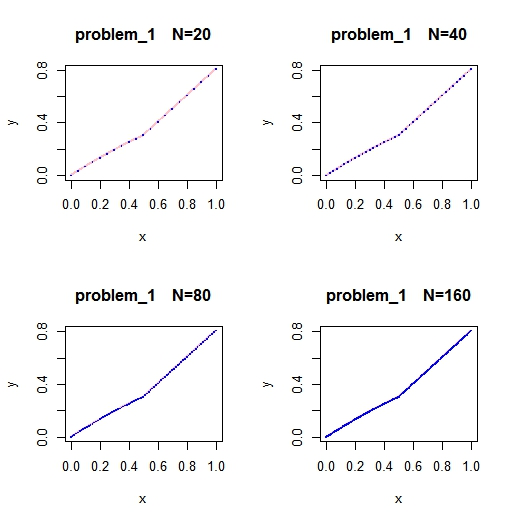
\includegraphics[width=1\textwidth,angle=0]{plot1.jpeg}
  \textbf {\caption{Solutions to problem1}}
\end{figure}
\newpage
The three norms of error function are tabled as below:
\begin{table}[ht]
\centering
\begin{tabular}{rrrrl}
  \hline
 N & max & L2 & H1 \\
  \hline
  20 &3.160035e-05 &7.677908e-05 &4.057766e-03 \\
  40 &7.898187e-06&1.919280e-05 & 2.028699e-03\\
  80 &1.974453e-06 &4.798084e-06 & 1.014326e-03\\
  160 &4.936576e-07 &1.199527e-06&5.071602e-04 \\
  \hline
\end{tabular}
\end{table}
\\In order to verify the assertion about the convergence rate, Let $log_2(N/20)$ be x-axes and $log_2(error)$ be y-axes, The graph is as follows:
\begin{figure}[htp]
  \centering
  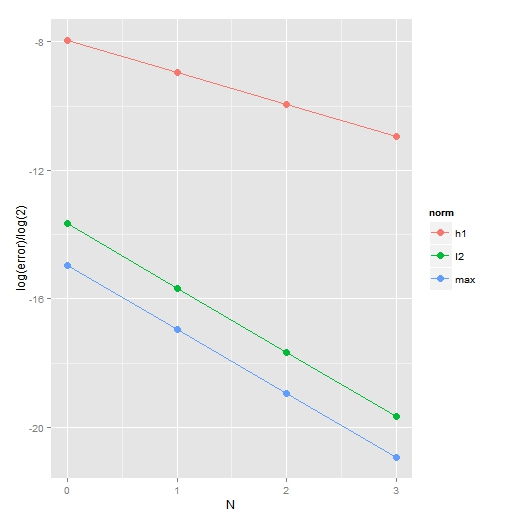
\includegraphics[width=0.5\textwidth,angle=0]{norm1.jpeg}
  \textbf {\caption{Error Changes}}
\end{figure}
\\It is easy to see in the picture that the max-norm and the L2-norm are at a scope of -2 and the H1-norm are at a scope of -1.



\section{problem2}
\subsection{Problem Specifications}
Consider the following problem:
$$W''(x)-\frac{F}{D}W(x)=-\frac{qx}{2D}(l-x),  x \in (0,l), W(l)=W(0)=0$$

$$
W(t) = \frac{b}{a}\{-t^2+t-\frac{2}{a}+\frac{2}{asinh(\sqrt{a})}[sinh(\sqrt{a}t)+ sinh(\sqrt{a}(1-t))]\}
$$

The real solution belongs to the functional space $H^1_0(0,1)$.
Let V = $\{v\in H^1(0,1), v(1)=v(l)=0\}$. We could rewrite the problem in a variational/weak form by partial integral calculus:
\\(V) Find $u \in V$ s.t \\
$$a(u,v)=L(v)$$
where
\begin{eqnarray}
a(u,v) &=& \int_0^l k(x)u'(x)v'(x)dx + \int_0^l u(x)v(x)dx \notag \\
L(v) &=& \int_0^l f(x)v(x)dx
\end{eqnarray}
\\where 
\begin{eqnarray}
f(x)&=& -\frac{qx}{2F}(l-x)\notag \\
k(x)&=& D/F;
\end{eqnarray}

The partition and generation of $V_h$ is similar to problem1 except that it is the family of $\{\phi_i\}_1^{N-1}$ that generate $V_h$ instead of $\{\phi_i\}_1^{N}$. And the definition of each $\phi_i$ is identical to that in problem1.
\\Thus $$V_n = span\{\phi_1...\phi_{N-1}\}$$ is a (N-1)-dimension functional space.
\newline Assume that $u_h(x)=\sum_1^{N-1}y_i\phi_i(x)$ solves equation(1) for every $v \in V_h$. What we want to get is the value of $\{y_i\}_i^{N-1}$. And we can generate a series of linear equations about $\{y_i\}_i^{N-1}$ from what we discussed above:\\
$$
\left\{
\begin{array}{rcl}
\int_0^1k(x)u_h'(x)\phi_1'(x)dx + \int_0^1u_h(x)\phi1(x)dx &=& \int_0^1f(x)\phi_1(x)dx\\
\int_0^1k(x)u_h'(x)\phi_2'(x)dx + \int_0^1u_h(x)\phi2(x)dx &=& \int_0^1f(x)\phi_2(x)dx\\
......& & \\
\int_0^1k(x)u_h'(x)\phi_{N-1}'(x)dx +\int_0^1u_h(x)\phi_{N-1}(x)dx &=& \int_0^1f(x)\phi_{N-1}(x)dx\\

\end{array} \right.
$$
We can get $\{y_i\}_i^N$ from the equation above thus we obtain the FEM solution.
\subsection{Results}
Our results of problem2:  
\begin{figure}[htp]
  \centering
  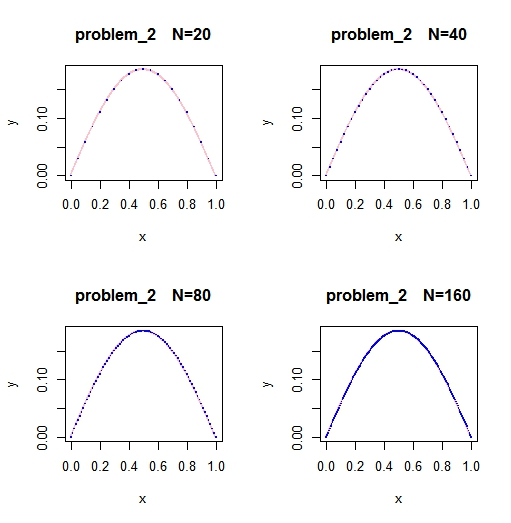
\includegraphics[width=1\textwidth,angle=0]{plot2.jpeg}
  \textbf {\caption{Solutions to problem2}}
\end{figure}
\newpage
The three norms of error function are tabled as below:
\begin{table}[ht]
\centering
\begin{tabular}{rrrrl}
  \hline
 N & max & L2 & H1 \\
  \hline
  20 & 1.091257e-07 &2.090290e-03 &3.371253e-03 \\
  40 &2.721892e-08 &5.227859e-04 & 1.422463e-03\\
  80 &6.858611e-09 &1.307105e-04 & 6.742980e-04\\
  160 &1.737309e-09 &3.267912e-05&3.323708e-04 \\
  \hline
\end{tabular}
\end{table}

\begin{figure}[htp]
  \centering
  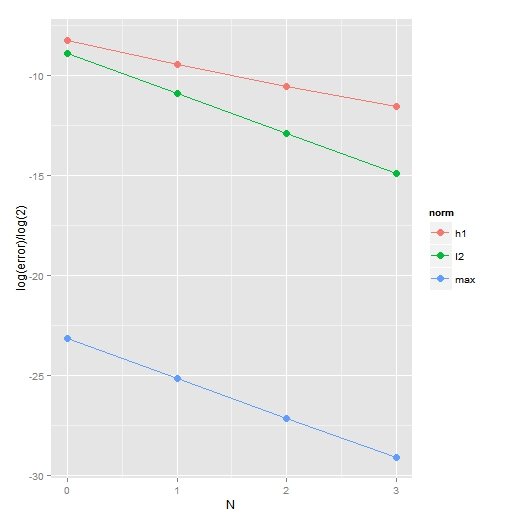
\includegraphics[width=0.5\textwidth,angle=0]{norm2.jpeg}
  \textbf {\caption{Error Changes}}
\end{figure}
\section{problem3}
As for problems3, firstly we should compute the solution in theory:
$$W(t) = A * t*t + B*t + C + D * sinh(sqrt{a}*t) + E*sinh(sqrt{a}*(1-t))$$
where\\
$$A = -b/a$$, $$B = b/a$$, $$C=-2b/a^2$$, 
$$D = b/(a\sqrt{a}cosh(\sqrt{a})) + 2b/(a^2cosh(\sqrt{a})sinh(\sqrt{a}))$$, 
$$E = 2b/(a^2/sinh(\sqrt{a}))$$.
\newline We can adopt almost the same method as that above to solve this problem. However, it most be noted that $$V_n = span\{\phi_1...\phi_{N}\}$$ is a N-dimension functional space.
\\So we can just give result without some trivial details:
\begin{table}[ht]
\centering
\begin{tabular}{rrrrl}
  \hline
 N & max & L2 & H1 \\
  \hline
  20 & 3.496205e-07 &2.088022e-03 &3.368619e-03 \\
  40 &8.741056e-08 &5.222187e-04 & 1.421528e-03\\
  80 &2.201801e-08 &1.305679e-04 & 6.738868e-04\\
  160 &5.769394e-09 &3.264236e-05&3.321726e-04 \\
  \hline
\end{tabular}
\end{table}

\begin{figure}[htp]
  \centering
  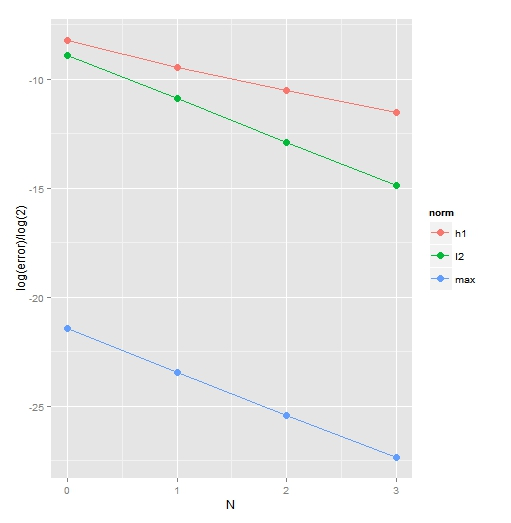
\includegraphics[width=0.5\textwidth,angle=0]{norm3.jpeg}
  \textbf {\caption{Error Changes}}
\end{figure}

\begin{figure}[htp]
  \centering
  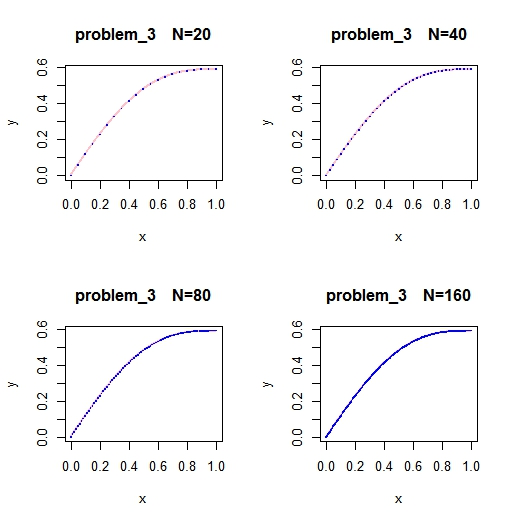
\includegraphics[width=1\textwidth,angle=0]{plot3.jpeg}
  \textbf {\caption{Solutions to problem3}}
\end{figure}
\newpage

\section{Conclusion and Discussion}
In our passage, we calculate the solution to a differentiate equation via linear nodal FEM. This assignment gives the detail implement of FEM and the solution to specific problem.
\\On the other hand, our results verify the theory prediction discussed in class:
$$
||u_h-u||_{L^{\infty}} \sim ch^2
$$
$$||u_h-u||_{L^2} \sim ch^2$$
$$||u_h-u||_{H^1} \sim ch
$$
\par Because if $||u_h-u|| \sim ch^{\alpha}$ (h=1/N),the scope of the graph in which $log_2(N/20)$ is x-variable and $log_2(||u_h-u||)$ is y-variable is about -$\alpha$
It is easy to see in the picture above that the max-norm and the L2-norm are at a scope of -2 and the H1-norm are at a scope of -1, which strongly support the prediction in class.
\par
Though this assignment, I practice my coding skills a lot and it is helpful for me to realize more about the conception and implement of FEM. In addition, when coding, I understand the difference of accurate between Gauss-method and Simpson-method. However, due to time limit, I can not complete the FEM using quadratic polynomials.









\end{document}